\documentclass{article}
\usepackage{graphicx} % Required for inserting images

\title{Who's fastest: a comparative study of four different sorting algorithms}
\author{Snehal Dutta}
\date{5th December 2023}

\begin{document}

\maketitle

\section{Introduction}
In this paper, we will examine a classical problem: sorting. The problem is to arrange an array of n integers according to some total order with a complexity of O(1). We use $<$ of total order.

This paper compares three comparison-based algorithms: Insertion sort, Quick Sort, and HeapSort, and one non-comparison-based algorithm: Radix Sort.

\subsection{Insertion Sort}
Insertion sort is a sorting algorithm that works efficiently with small datasets.

Insertion sort computes by taking an array as a parameter which stores a sequence of n numbers to be sorted. Then it iterates over the array and compares the current element(key) to its predecessor, if the key is smaller than its predecessor then we compare it with elements before it. The greater elements are positioned in one place up to make space for the swapped elements.

The best-case time complexity is $0(n)$ when the array is sorted in ascending order.
The worst-case time complexity is $0(n^2)$ when the array is sorted in descending order.
The average time complexity is $0(n^2)$.
The algorithm is stable and in place.

\subsection{Quicksort}
Quicksort is a comparison-based sorting algorithm that works on the Divide and divide-and-conquer method. 

The algorithm picks one element as the pivot and partitions the array in and around the pivot by placing the pivot in the correct position in the sorted array. Firstly, Quicksort divides the array (partition) into two possibly empty sub-arrays such that the elements of the left sub-array are less than the pivot index which is smaller or equal to the elements of the right sub-array. Then, finally, we return the value of the pivot index. After dividing, we start sorting the sub-arrays by recursively calling the quicksort. Finally, we combine both the sub-arrays to get a sorted array.

The best-case time complexity is $0(nlogn)$ when the pivot is chosen as the mean.
The worst-case time complexity is $0(n^2)$ when the array is not divided into equal parts i.e.; one being $(n-1)$ and the other and so on.
The average time complexity is $0(nlogn)$ when the array is divided into two parts i.e.; $k and (n-k)$.

The algorithm is not stable but in place.
\subsection{Heap Sort}
Heap Sort is a comparison-based sorting algorithm that is based on heap data structure. Each node of the heap corresponds to an index of the array.

Firstly, we have to convert the array into a heap using the heapify function keeping the greatest element as the root node. Then we delete one by one root node of the max-heap and replace it with the last node of the heap and then again heapify the root of the node. We have to continue the process till the size of the heap is greater than 1. 

The best-case time complexity is $0(nlogn)$.
The worst-case time complexity is $0(nlogn)$.
The average-case time complexity is $0(nlogn)$.

The algorithm is not stable but in place.
\subsection{Radix Sort}
Radix Sort is a non-comparison linear sorting algorithm mainly efficient in sorting integers and strings of fixed-size keys.

The key idea of the Radix Sort algorithm is to exploit the concept of place value. The algorithm sorts the elements by processing them digit by digit. Rather than comparing elements directly, Radix Sort distributes elements into buckets based on the digit's value. By repeatedly sorting the elements by their significant digits, from the least significant to the most significant, Radix sort achieves the final sorted list.

The best-case time complexity is $0(d*(n+b))$ where d is the number of digits, n is the number of elements and b is the base of the number system used.
The best-case time complexity is $0(nlogn)$ 
The best-case time complexity is $0(nlogn)$ 

The algorithm is stable but not in place.

\section{Methodology}
The algorithms are implemented in Python.
The results are generated in two categories: sorted arrays (best case for insertion sort) and randomly shuffled arrays of values $0$, $1$, $2$, \dots, $n-1$

The algorithms are tested on array size consisting of $1$,$2$,$3$, \dots, 10000.
In both categories, each algorithm is given the same input data.
Each array size is tested 100 times.

The result for each size is the average time taken by each algorithm to sort the input array.
\section{Results}

\begin{figure}[ht]
\centering
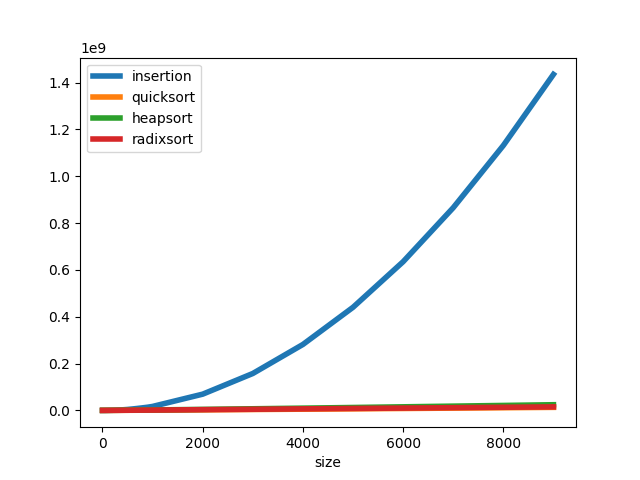
\includegraphics[width=0.8\linewidth,height=0.4\textheight]{plt1.png}
\caption{Average time each algorithm took to sort an array of randomly shuffled values from $0$ to $n - 1$.}
\label{avg}
\end{figure}

\begin{figure}[ht]
\centering
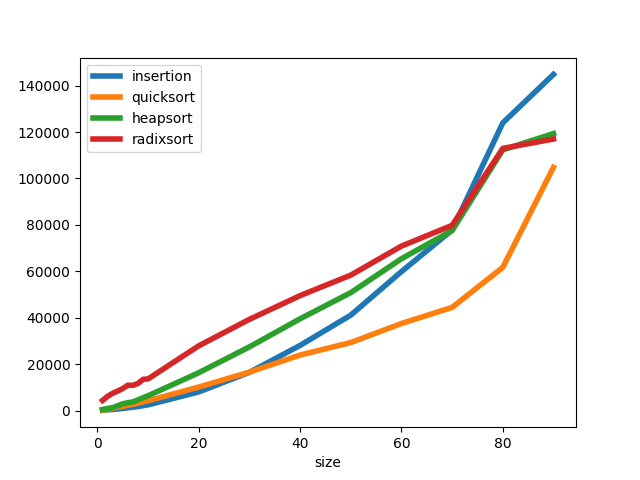
\includegraphics[width=0.8\linewidth,height=0.4\textheight]{plt5.png}
\caption{The graph shown in Figure \ref{avg} for small array sizes.}
\label{avg:small}
\end{figure}

Graphs of results for the average case of all sorting algorithms are represented in Figures \ref{avg} and \ref{avg:small}.
Insertion Sort takes several times longer than any other algorithm.
Initially, in small datasets insertion sort performed efficiently but eventually, quicksort performed the best.

\begin{figure}[ht]
\centering
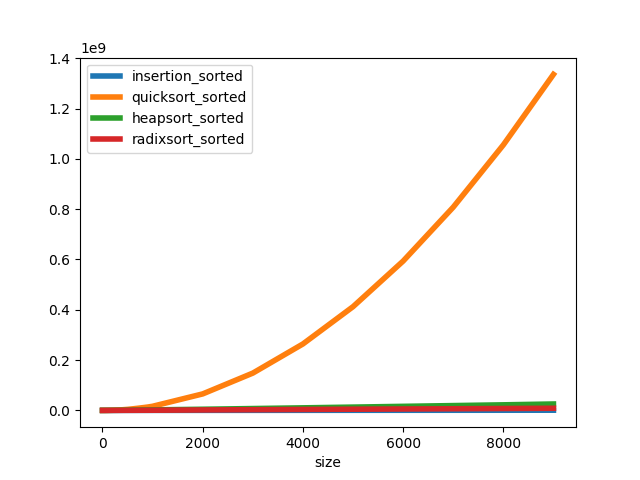
\includegraphics[width=0.8\linewidth,height=0.4\textheight]{plt2.png}
\caption{Average time each algorithm took to sort an array of sorted values }
\label{best}
\end{figure}

\begin{figure}[ht]
\centering
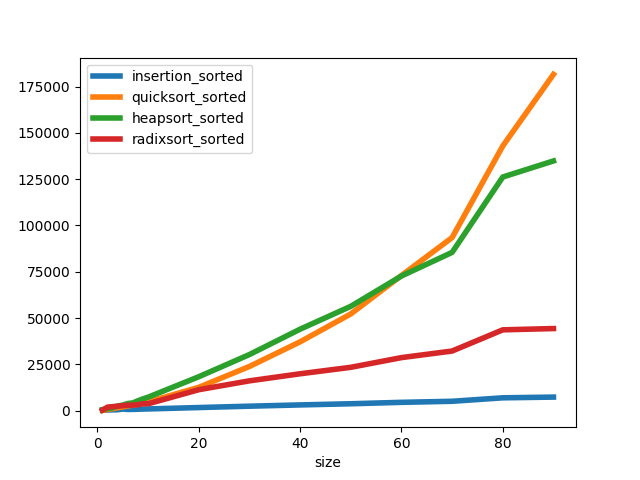
\includegraphics[width=0.8\linewidth,height=0.4\textheight]{plt6.png}
\caption{The graph shown in Figure \ref{best} for small array sizes.}
\label{best:small}
\end{figure}

Graphs of results for the average time to sort a sorted array of all sorting algorithms are represented in Figures \ref{best} and \ref{best:small}
In both the graphs, Insertion sort performed the best among all the algorithms as it is the best-case. On the contrary, quicksort performed worst as the arrays were not perfectly divided into two parts. Thus, it's the worst case. 

\begin{figure}[ht]
\centering
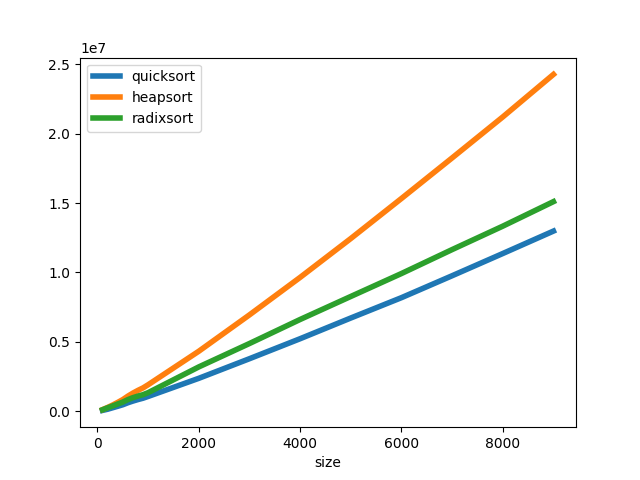
\includegraphics[width=0.8\linewidth,height=0.4\textheight]{plt3.png}
\caption{Average time each algorithm took to sort an array of randomly shuffled values from $0$ to $n - 1$. excluding insertion sort}
\label{avg1}
\end{figure}
\begin{figure}[ht]
\centering
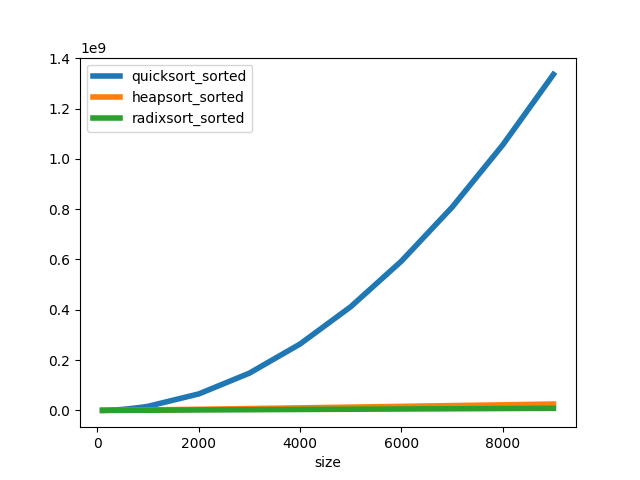
\includegraphics[width=0.8\linewidth,height=0.4\textheight]{plt4.png}
\caption{Average time each algorithm took to sort an array of sorted values excluding insertion sort.}
\label{avg1:best}
\end{figure}

Graphs of results for the average time to sort a randomly shuffled array and a sorted array of all sorting algorithms respectively are represented in Figures \ref{avg1} and \ref{avg1:best}.
In figure \ref{avg1}, Quicksort and Radix Sort are almost close to each other but Quicksort was faster than the RadixSort. HeapSort did not perform faster in this case.
QuickSort was approximately 0.0025\% faster than Radix Sort.
\section{Conclusion}
We conclude that QuickSort is the best among the four sorting algorithms.
\end{document}
